\documentclass[twocolumn]{article}
\usepackage[utf8]{inputenc}
\usepackage{polski}
\usepackage{amsmath}
\usepackage{amsfonts}
\usepackage{float}
\usepackage{fancyvrb}
\usepackage{multicol}
\usepackage{enumitem}
\usepackage{listings}
\usepackage{textcomp}
\usepackage{wasysym} % TODO: using for \natural, find better package instead
\usepackage[a4paper, total={8in, 10in}]{geometry}
\setlength{\columnseprule}{0.0001pt}
\lstset{
  basicstyle=\ttfamily,
  mathescape
}

\title{Algorithmic Aspects of Game Theory}
\author{Tomasz Garbus}
\date{2019}

\usepackage{natbib}
\usepackage{graphicx}

\begin{document}
\renewcommand{\contentsname}{Contents}
\renewcommand{\figurename}{Fig.}

\maketitle
\tableofcontents

\section{Lecture 1 (27 II 2019)}

\section{Tutorials 1 (28 II 2019)}
Hex, choquet: 2 players.\\
We say a game is \textbf{determined} if either of players has a winning
strategy,
If $\sigma$ is a winning strategy of $P$, then $\forall_{\pi} G(\sigma, \pi) \leftarrow$ wins $P$.\\

\noindent
\textbf{1.} Is the choquet game determined if we replace $\mathcal{R}$ with $\mathcal{Q}$ (and its topology)?\\
If so, who has a winning strategy?\\

\noindent
\textbf{2.} Let's consider a variant of choquet games on topological spaces. We have a property:
If $X$ is not a Baire space\footnote{$X$ is Baire \underline{if}:\\
$G_i \leftarrow$ are dense and open for $i \in \mathcal{N}$
then $\cap_{i > 0} G_i \neq \emptyset$\\
}
$\implies$ $E$ has a winning strategy (E means Empty, not Eve!).\\
Example with rational numbers:\\
$G^q \leftarrow$ set $\mathcal{Q} \setminus {q}$ dense, open.\\
$Q$ is countable.\\
$F \subset Q$\\
$\cap_{q \in F} G^q = G^F$\\
$|F| < \mathfrak{c}$\\
Our strategy:
\begin{itemize}
	\item we start with set $G^{q_0}$
	\item opponent plays a set, say $S_1$
	\item we play a set $S1 \cap G^{q_0} \cap G^{q_1}$
\end{itemize}

\noindent
\textbf{3.} If $X$ is complete then $NE$ has w.s.\\
A complete space is also a Baire space.\\

\noindent
\textbf{4.} Consider \textsc{Nim} game.\\
Setup: $n$ heaps with tokens $h_1, h_2, ..., h_n$.\\
Move: choose a heap and remove $r > 0$ tokens.\\
Win: The last move.\\
We have two players: \textsc{E} and $\forall$, Eve move first.
Q: Who has a winning strategy? When is the game determined?\\

\noindent
$n = 1 \leftarrow$ Eve always wins\\
$n = 2 \leftarrow$ ((1, 1) wins Adam, (2, 1) wins Eve, (2, 2) wins Adam)
($h_1$, $h_2$) $\rightarrow$ equalise them if possible\\
Eve has a winning strategy iff $h_1 \neq h_2$\\
General case: Eve wins if the xor of stack heaps is non-zero. Proof: The winning configuration has xor 0.
From a situation with xor $\neq 0$ is always able to produce a situation with xor $ = 0$ and if xor $ = 0$,
it's impossible to make a move such that xor $ = 0$ after the move.\\
\begin{itemize}
	\item[1] $(0, ..., 0, h_j, 0, ..., 0)$ is a winning position for Eve.
	\item[2] if $h_1 \otimes h_2 ... \otimes h_n = 0$ then the position is \textit{balanced}.
	Balanced positions are winning positions.
	\item[3] Show strategy (next tutorials)
\end{itemize}

\section{Lecture 2 (6 III 2019)}
\subsection*{Determinacy}
If we have a \textbf{game of finite duration} with 2 players, we can expand the
game in a tree, where a leaf signifies the end of the game. A leaf maps to one of
three possible situations:
\begin{itemize}
	\item existential player ($\exists$) wins
	\item universal player ($\forall$) wins
	\item draw
\end{itemize}
If we map those situations to values accordingly: $1, -1, 0$, the existential
player aims to maximize (and universal to minimize) the outcome value.\\

\noindent
Let's consider \textbf{infinite} games now. Suppose we have 2 players and draw is
not possible in the game. If the player does not know the winning strategy, it is
possible that they may "loop" in a position with winning strategy but never proceed
with it.\\

\noindent
There \textbf{exist} indeterminate perfect information games.\\

\noindent
Infinite XOR game: $E$ and $A$ alternately play words $w_0, w_1, w_2, ... \in \{0, 1\}^{+}$
which are concatenated to $w_0w_1w_2...$.\\

\noindent
Infinite XOR: any function $f: \{0, 1\}^{|\mathbb{N}|} \rightarrow \{0, 1\}$ such that
if $v, w$ differ by one bit then $f(v) \neq f(w)$.\\
$v \sim w$ iff differ by a finite number of bits.\\
We can choose set $S$ s.t. $\{0, 1\}^{|\mathbb{N}|} \supseteq S$ has $\exists!$ element for each equivalence class (from \textit{Axiom of Choice}).\\
Each equivalence class of $\sim$ is countable, thus there is continuum of equivalence classes.

\noindent
Eve wins iff $f(w_0w_1...) = 0$, Adam otherwise. No player has a winning strategy
in this game.\\
\underline{1. Suppose Adam wins.} In the first play:
\begin{verbatim}
E  0      w_2       w_4
A    w_1       w_3
\end{verbatim}
Then in the next game Eve can steal his strategy:
\begin{verbatim}
E  1 w_1        w_3       w_5
A         w_2        w_4
\end{verbatim}
\underline{2. Suppose Eve wins.} In the first play:
\begin{verbatim}
E  w_0    w_2      w_4
A       0      w_3
\end{verbatim}
Then in the next play:
\begin{verbatim}
E  w_0         w_3
A       1 w_2       w_4
\end{verbatim}

\subsection*{Game on graph}
An \textit{arena} is a directed graph, consisting of:
\begin{itemize}
	\item the set of \textit{positions} $Pos$
	\item the set of \textit{moves} $Moves \subseteq Pos \times Pos$
\end{itemize}
$Pos = Pos_{\exists} \cup Pos_{\forall}$,\\
$Pos_{\exists} \cup Pos_{\forall} \neq \emptyset$.\\
A \textit{play} is a finite or infinite sequence of moves:\\
$q_0 \rightarrow q_1 \rightarrow q_2 \rightarrow ... \rightarrow q_k (\rightarrow ...)$.\\

\noindent
\underline{Game equation}
\begin{figure}[H]
	\centering
	$X = (E \cap \diamond X) \cup (A \cap \square X) = Eve(X)$\\
	$Y = (E \cap \square Y) \cup (A \cap \diamond Y) = Adam(Y)$
\end{figure}
\noindent
$E = Pos_{\exists}$,\\
$A = Pos_{\forall}$,\\
$X, Y \in \mathcal{P}(Pos)$\\
"Modal logic" symbols here:\\
$\diamond Z = \{p : (\exists_q) Moves(p, q) \land q \in Z\}$
\footnote{
	$p \rightarrow q$ also denotes $Moves(p, q)$ below.
	A position $p$, such that $(\forall_p) p\not\rightarrow q$ is called \textit{terminal},
	which we also write $p \not\rightarrow$.
}\\
$\square Z = \{p : (\forall_q) (p \rightarrow q) \Rightarrow q \in Z\}$\\

\noindent
\textbf{Knaster-Tarski Theorem}: $\langle L, \le \rangle$ complete lattice\footnote{
	A \textit{complete lattice} is a partially ordered set $\langle L, \leq \rangle$, such that
	each subset $Z \subseteq L$ has the least upper bound $\bigvee Z$, and the greates lower
	bound $\bigwedge Z$. In particular, $\bigvee \emptyset$ is the least element denoted $\bot$,
	and $\bigwedge \emptyset$ is the greatest element denoted $\top$.
}, $f : L \rightarrow L$ monotonic,
then there exists a least fixed point\\
$\mu x. f(x) = \bigwedge \{d : f(d) \leq d\}$ and a greatest fixed point:\\
$\nu y. f(y) = \bigvee \{d : d \leq f(d) \}$.\\
\textbf{Proof}: We show the proof for the greatest fixed point. Let $a = \bigvee A, A = \{z : z \leq f(z)\}$\\
Because $f$ is monotonic, $z \leq a$ implies $f(z) \leq f(a)$. For $z \in A$, this also means $z \leq f(z) \leq f(a)$.
Hence, $f(a)$ is an upper bound of $A$, which follows $a \leq f(a)$. Using the monotonicity of $f$ once more, we obtain
$f(a) \leq f(f(a))$. Hence $f(a) \in A$, which follows the converse inequality $f(a) \leq a$.\\

\noindent
We consider mappings $Eve$ and $Adam$ defined in the complete lattice $\langle \mathcal{P}, \leq \rangle$.
$Eve(Z)$ is a set of such positions from which Eve can win, and $Adam(Z)$ is a set of such positions from which Adam can win.

\subsection*{Traps and gardens of Eden}
\noindent
A set of positions $Z \subseteq Pos$ is a trap for Adam if $Z \subseteq Eve(Z)$. It means that Adam cannot go out of there.\\
A set of positions $Z \subseteq Pos$ is Garden of Eden for Eve if $Eve(Z) \subseteq Z$. It means that Adam cannot enter those positions.\\

\noindent
The \textit{greatest} trap for Adam is a garden of Eden for Even.\\
The \textit{least} garden of Eden for Eve is a trap for Adam.\\

We use the notation: $\overline{Z} = Pos - Z$.

\subsubsection*{Lemma}
\begin{figure}[H]
	\centering
	$\overline{Eve(X)} = Adam(\overline{X})$
\end{figure}
\textit{Proof.} We have:\\
$\overline{Eve(X)} = \overline{(E \cap \diamond X) \cup (A \cap \square X)}\newline
 = (\overline{E \cap \diamond X}) \cap (\overline{A \cap \square X})\newline
 = (\overline{E} \cup \overline{\diamond X}) \cap (\overline{A} \cup \overline{\square X})\newline
 = (A \cup \square \overline{X}) \cap (E \cup \diamond \overline{X})\newline
 = (A \cap \diamond \overline{X}) \cup (E \cap \diamond \overline{X})
 \cup (A \cap E) \cup (\diamond \overline{X} \cap \square \overline{X}) = Adam(\overline{X})$\\

\noindent
\underline{\textbf{Proposition:}} $Pos$ can be divided to three disjoint sets:
$\mu X. Eve(X)$, $\mu X. Adam(X), (\nu Y. Eve(Y)) \cap (\nu Y. Adam(Y))$\\

\subsection*{Definition: strategy}
A strategy (for Eve) is a set of finite plays s.t.:
\begin{itemize}
	\item if $last(w) \in Pos_{\exists}$ then $\exists! q$ s.t. $last(w) \rightarrow q$ and $wq$ is in $S$
	\item if $last(w) \in Pos_{\forall}$ then $\forall(q) (last(w) \rightarrow q) \Rightarrow wq \in S$
	\item $S$ is closed under initial segments, i.e., if $s_0s_1...s_k \in S$, then $s_0s_1...s_i \in S$,
	for $0 \leq i \leq k$j
\end{itemize}

\section{Tutorials 2 (7 III 2019)}
\noindent
\textbf{1.} Consider \textsc{Nim} game.\\
We have $n$ stacks of heights $h_1, h_2 ..., h_n, h \in \{0, 1, 2, ...\}$.\\
$W_E = \{x \in \mathbb{N}^R : \text{Eve has a w.s.}\}$.\\
Let's take $x \in \mathbb{N}^R, x = (h_1, ..., h_n)$.\\
$h_1^b \otimes h_2^b \otimes ... \otimes h_n^b \neq 0 \rightarrow \text{Eve wins from } x$.\footnote{($h^b$ means binary representation)}\\
The proof consists of 3 observations:
\begin{itemize}
	\item Final position (all empty stacks) has xor equal to 0.
	\item From a position s.t. xor $\neq 0$, it is always possible to zero the xor.
	Let xor be equal some $y$. Let $d$ be the position of leftmost (most important)
	bit in binary representation of xor. Thus in some stack, the binary representation
	must have The $d$-th bit activated. We can then deactivate $d-$th bit and set
	appropriate values on all less significant bits (to zero the xor), and the resulting
	stack height will be lower.
	\item From a position s.t. xor $= 0$, all moves lead to xor $\neq 0$. If we take
	a non-zero number of tokens from a stack, it means we alter a non-zero number of
	binary digits in the representation of xor, thus it is no longer 0.
\end{itemize}
Thus, $W_E = \{x \in \mathbb{N}^R : \otimes x \neq \vec{0}\}$.\\

\noindent
\textbf{2.} Represent \textsc{Nim} as a game on graph.\\
The set of positions is the set of all stack configurations. In general, the space of positions is infinite,
but for a fixed game we have finite set of positions.\\
However, this is not enough (in a game on graph, we want $Pos$ to be disjoint set $Pos = Pos_E \cup Pos_A, Pos_E \cap Pos_A = \emptyset$).
Thus we also add information who moves next.\\
Graph: $G = \langle V_E \dot\cup V_A, E \rangle$.\\
Strategy is a function $\sigma : V^*V \rightarrow V$, $\sigma(v_0v_1v_2...v_nv_{n+1}) \rightarrow v$.\\
Let $w = v_1...v_n...$ be a winning position. We say that first player wins if their strategy $L \in V^{w}$.\\
In \textsc{Nim}, the winning condition does not depend on history, so we can collapse the states with the same stacks configuration in the last move
(and of course the same currrent player).\\

\noindent
\textbf{3.} Chocolate game.\\
We have a grid $m \times n$. A player chooses a field and everything on the right and up
is erased. One restriction: you cannot choose position $(1, 1)$. The player who makes last
move wins.
\footnote{
Other definition: players eat chocolate, position $(1, 1)$ is poisoned.
}
Is the game determined? Who has a winning strategy?
\begin{itemize}[leftmargin=*,labelindent=12.5mm]
	\item[$1 \times n$:] Eve wins (obvious)
	\item[$2 \times n$:] Eve wins: she eats the position $(n, 2)$ and always maintains
	the bottom row has one piece more than the top one.
	\item[$\omega \times \omega$:]\footnote{$\omega = \{0, 1, ...\}$} Eve wins: eat the position $(2, 2)$ and then maintain $(1, n); (n, 1)$
	\item[$m \times n$:]\footnote{$m, n \in \mathbb{N}$} Assume the $2$nd player wins. That means that for
	any move made in the first move, there exists such move from a second player, that the second player
	has a winning strategy after the second move.\\
	We can use a strategy stealing argument: First player removes a rectangle larger than $1 \times 1$.
	Then by assumption the second player has a winning strategy. But instead we can start by removing
	only one piece of chocolate. Then second player must make a move such that only a single rectangular
	area is removed (which could be made in one move by the first player). Then first player can copy
	second player's winning strategy. Thus second player does not have a winning strategy.\\
\end{itemize}
Above we have shown that the second player has no w.s.\\
$\lnot \exists_{\pi} \forall_{\sigma} \pi \text{ wins with } \sigma \Leftrightarrow \forall_{\pi} \exists_{\sigma} \sigma \text{ wins with } \pi$.
But this doesn't imply $\exists_{\sigma} \forall_{\pi} \sigma > \pi$ (although there is an implication the other way).\\
We will just show the game is determined, without showing the winning strategy:\\
We can build the graph of positions. All paths from $m \times n$ (starting position)
are finite, the size of graph is finite as well. We can thus infer the winning position by
searching the graph bottom-up (from node $0, 0$ to $m, n$). We have thus shown the game is
determined for a finite size. Since Adam does not have a winning strategy, thus Eve must have
it.\\
For $\omega \times \omega$ we use an argument that after the first move the game graph must have
a finite height.\\

At home: think about chess determinacy, also Armageddon version (black wins if he doesn't lose, also for draw).

\section{Lecture 3 (13 III 2019)}

Arena: $Pos = Pos_E \dot\cup  Pos_A$\\
Move $\in Pos \times Pos$\\

\noindent
\textbf{Zermelo}: in chess, either White or Black have winning strategies, or
both have a strategy for a draw (at least).\\
\textbf{Theorem}: In a graph game, for each position $\gamma$ either Eve has a
strategy to win in finite time, or Adam has a strategy to win in finite time,
or both have strategies to survive. Moreover, all strategies can be positional
\footnote{
	A strategy $S$ is \textit{positional} (or \textit{memory-less}) if this
	function depends only on the current position.
}.\\
Strategy (for Eve): \textit{I will tell you what to do if you have obeyed me so
far.}\\
for $w \in S$:\\
if $last(w) \in Pos_E$ then $(\exists !p) wp \in S$\\
if $last(w) \in Pos_A$ then $(\forall p) ((last(w) \rightarrow p) \Rightarrow wp \in S)$\\

\noindent
Strategy $S$ is positional (memory-less) if $last(w) = last(v)$ then $f_s(w) = f_s(v)$.\\

\noindent
$f_S$ can be viewed as a partial function on positions of Eve.\\

\noindent
If $X \subseteq Eve(X)$ then any function $dom_f = X \cap Pos_E$ such that $(\forall x \in dom_f) f(x) \in X$
witnesses the trap $X$.\\
A function is safe if it is a witness of a trap.\\
\underline{\textbf{Prop.}} A partial function $f : Pos_E \supseteq dom_f \rightarrow Pos$
is $f_S$ for some positional strategy iff \underline{it is safe}. Moreover if $f$ is a witness of trap $Z$ then
$f = f_S$ such that $start(S) = Z$\footnote{
$Start(S) = S \bigcap Pos$
}.\\

\noindent
\underline{\textbf{Proof}}: Suppose $f$ is a witness for trap $Z$. We define $S = \bigcup_{n = 0} S_n$,
$S_0 = Z$, $S_n$\\

\noindent
A position $p$ is safe for Eve if $p \in S$ for some strategy for Eve.\\
\textbf{Lemma 1} $Safe_E$ -- the set of all safe positions for $E$. $Safe_E = \nu X . Eve(X)$.
Moreover, Eve has a positional strategy $S$, with $start(S) = Safe_E$.\\
\textbf{Lemma 2} $Win^{fin}_{E}$ -- the set of positions, from where Eve can win in finite time.
Then $Win^{fin}_{E} = \mu x. Eve(X)$. Moreover Eve has a positional strategy $S$ finitely winning
with $Start(S) = Win^{fin}_{E}$.

\noindent
\textbf{Proposition (from Lecture 2)} \textit{The complement of a trap for Adam is a garden of Eden for him; similarly for Eve.}\\
\textbf{Proposition (from Lecture 2)}\\
$\overline{\mu X . Eve(X)} = \nu Y . Adam(Y)$\\
$\overline{\nu X . Eve(X)} = \mu Y . Adam(Y)$

\noindent
\textbf{Exercise (from Lecture 2)} \textit{Show that the union of any family of traps for a player is again a trap for this player. Note that this
implies that the intersection of any family of gardens of Eden for a player is again a garden of Eden for this player. Which more general property
of ordered sets underlines these facts? (Remember the Knaster-Tarski Theorem.)}\\
From definition, a set of positions $Z \subseteq Pos$ is a trap for Adam if $Z \subseteq Eve(Z)$. Let $ZS = Z_1, Z_2, ...$ be a (not necessarily finite)
family of traps. For every $Z_i$ and position $p \in Z_i$, $p \in Eve(ZS)$, thus $ZS \subseteq Eve(ZS)$ so we arrive to the definition of trap again.

\section{Tutorials 3 (14 III 2019)}
Ordinal numbers:\\
$0, 1, ..., \omega, \omega+1, ..., \omega+n, ... 2 \omega, ..., n \omega, \omega^2, ..., \omega^5, ..., \omega^\omega, ...$\\
$\alpha$\ \ \ $\alpha + 1$\ $|$\ $\alpha \cup \{\alpha\}$  $0 = \{\}$\\
Set of ordinals is well founded (no infinite descending sequence).\\
$\beta$\ \ \ $\bigcup\limits_{\alpha < \beta} \alpha$\\

\noindent
\textbf{1.} \textsc{Nim} on ordinals. $G = (h_1, .., h_n), h_i < \omega^\omega$.
\begin{itemize}
	\item[1)] Is $G$ determined (for which starting positions)?
	\item[2)] If so, who has a winning strategy?
\end{itemize}
1. \underline{Yes.} A graph of states is a DAG and can be divided into disjoint states of winning positions for both players.\\
2.
\begin{itemize}
	\item[a)] $h < \omega^\omega$\\
		$h = a_0 + a_1\omega + a_2\omega^2 + ... + a_n\omega^n\ \ (a_i \in \mathbb{N})$ (it is easy to show that this fits under $\omega^\omega$)\\
		In finite case ($a_i = 0$ if $i > 0$) we aim to zero the xor of all stacks. We will try to apply this strategy to ordinals. Let's
		define xor on ordinals.\\
		$\alpha, \beta$ -- ordinals\\
		$\alpha \oplus \beta = (\alpha_0 \oplus \beta_0) + (\alpha_1 \oplus \beta_1)\omega + ... + (\alpha_n \oplus \beta_n)\omega^n$\\
		\underline{Statement} In game $G = (h_1, .., h_n)$ Eve has a winning strategy iff $\underset{i > 0}{\oplus} h_i \neq \emptyset$.
		We need to prove that:
		\begin{itemize}
			\item[1\textdegree] If Eve plays from $\oplus \neq 0$ then she can always maintain $\oplus = 0$.
			\item[2\textdegree] $\oplus = 0 \Rightarrow$ Every Adam's move makes it $\neq 0$.
			\item[3\textdegree] Ends after a finite number of steps in necessarily Adam's position.
		\end{itemize}
\end{itemize}

\noindent
\textbf{2.} Infinite XOR is an undetermined game such that its graph of positions has inifinite branching. Try to find a game such that
is undetermined but has finite branching.\\
We modify the game so that player can only place a single letter from the alphabet $\Gamma = \{0, 1, 2, 3, \#\}$ and we have an interpretation function
$f : \{0, 1, 2, 3, \#\}^\omega \rightarrow \{0, 1\}^\omega$. If a player does not place a hash (end of a word) in a finite time, they lose. Once a player
places a hash, its the other player's turn.\\

\noindent
\textbf{Gale-Stewart games}: $\langle \Gamma, W \subseteq \Gamma^\omega \rangle$, game of perfect information.\\

\noindent
\textbf{Zermelo}: Let $G = \langle V, \rightarrow \rangle$ be a graph game. Then there exists a partition $W_E \dot\cup W_A \dot\cup W_N = V$
s.t. player $P \in \{E, A\}$ has a \underline{positional} winning strategy in position $v \in W_P$.\\

\noindent
\textbf{Reachability game}: We select a node in graph, Eve wants to reach that node, Adam does not want to ever reach that node. If the play is infinite and looped
without reaching the selected node, Adam wins.

\section{Lecture 4 (20 III 2019)}
\underline{Generalized Zermelo Theorem}: For any position $p$ in a deterministic, two-person game with perfect information (and players make moves alternatingly):
\begin{itemize}
  \item one of the players has a winning strategy (winning in finite time)
  \item or both players have a surviving strategy
\end{itemize}
Moreover, those strategies can be positional.\\
$Eve(X) = (E \cap \diamond X) \cup (A \cap \square X)$ -- those positions,
from which $X$ can be achieved in one move. If it is Eve's move, there must be
one move to position in $X$, if Adam's -- all moves must lead him to $X$.\\
We want to find the smallest fixed point $\mu X. Eve(X)$.\\
$\bigvee f^{\zeta}(\bot) = \mu x. f(x) = \bigwedge \{ d\ :\ f(d) \leq d\}$\\
$\bot$ -- minimal element\\
$f^0(\bot) = \bot$\\
$f^{\zeta + 1}(\bot) = f(f^{\zeta}(\bot))$\\
$\eta$ -- limit element:\\
$f^{\eta}(\bot) = \underset{\zeta < \eta}{\bigvee} f^{\zeta}(\bot)$\\

\noindent
Algorithm for finding winning positions for player $X \in \{Eve, Adam\}$:
\begin{lstlisting}[tabsize=2]
Program Win(X)    $X \in \{Eve, Adam\}$
W : Pos $\rightarrow \{ \bot, \exists, \forall \}$
Forall $p \in Pos$
 W(p) = $\bot$
 pred(p) = $\emptyset$
 nb(p) = 0
Forall (p, q) $\in$ Move
 pred(q) := pred(q) $\cup$ {p}
 nb(p) := nb(p) + 1
Forall p $\in$ Pos$_{\overline{X}}$
 if nb(p) = 0 then Propagate(p, X)

Propagate(q, X)
 if W(q) = $\bot$ then W(q) = X
 Forall p $\in$ pred(q)
  if W(p) = $\bot$ then
	 if p $\in$ Pos$_{X}$ then
    W(p) = X
    Propagate(p, X)
   else (* p $\in$ Pos$_{\overline{X}}$ *) then
    nb(p) := nb(p) - 1
	  if nb(p) = 0 then
	   Propagate(p, X)
\end{lstlisting}

\subsection*{Parity games}
$Pos_E, Pos_A, Move, rank : Pos \rightarrow C$\\
$Win_E \subseteq C^{\omega}$\\
$Win_A \subseteq C^{\omega}$\\
$Win_E \cap Win_A = \emptyset$\\
Parity games: $C \subseteq \mathbb{N}$\\
$Win_E = \{ u \in C^{\omega}\ :\ \underset{n \rightarrow \infty}{\lim\sup}\ u_n\ \text{is even} \}$\\
$Win_A = \overline{Win_E}$\\
Every position is winning for one of the players, with a positional strategy.

\section{Tutorials 4 (21 III 2019)}
A game $G = \langle B, W \rangle$\\
$B = \langle V, E, \lambda, v_I \rangle$\\
$E \subseteq V$, $\lambda\ :\ \rightarrow \Gamma$, $v_I \in V$\\
$W \subseteq \Gamma^{*} \cup \Gamma^{\omega}$\\
$\Phi\ :\ \Gamma^{\omega} \rightarrow [0, 1]$\\
$\Phi_W(x) = \begin{cases}
1,\ x \in W\\
0,\ x \not\in W
\end{cases}$\\

\noindent
Example:
\begin{figure}[H]
	\centering
	\caption{Consider this simple game on graph}
	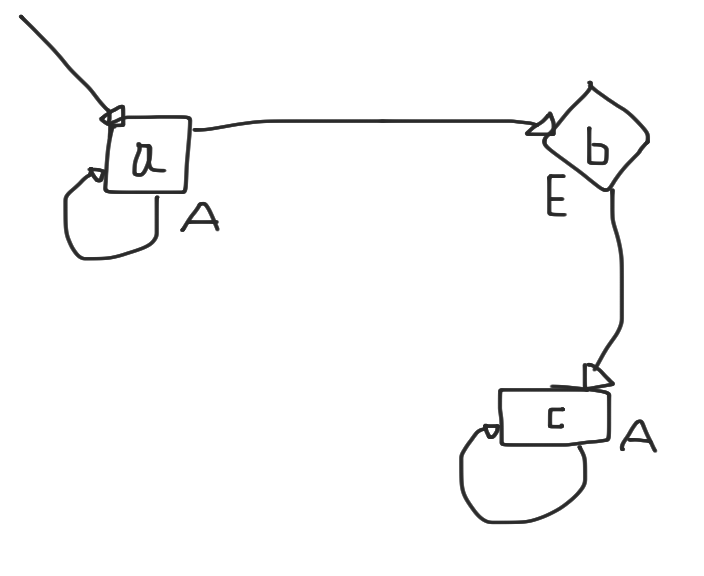
\includegraphics[scale=0.2]{content/graphics/game1.png}
\end{figure}
\noindent
$W = \{w \in \{a, b, c\}^{\omega}\ |\ \exists_{n < \omega} w = a^nb^nc^{\omega}\}$ -- Adam has a winning strategy
(he can infinitely loop in \texttt{a}).\\

\noindent
Strategies for Eve and Adam:\\
$E:\ \delta\ :\ V^{*}V_E \rightarrow V$ s.t. $\delta(w, v) \rightarrow (v')$ (and $v,v' \in E$)\\
$A:\ \pi\ :\ V^{*}V_A \rightarrow V$\\
Or positional strategies:
$\delta\ :\ V_E \rightarrow V$\\
$\pi\ :\ V_A \rightarrow V$\\
A play:\\
$G<\delta, \pi> \rightarrow v_0v_1v_2...v_n.... = p$\\
$w = \lambda(v_0)\lambda(v_1)...\lambda(v_n)...$\\
$w \in W \Leftrightarrow \delta\text{ wins with }\pi$\\

\noindent
(still considering the game above)\\
$W_2 = W \cup \{a^{\omega}\}$ -- Eve has a winning strategy (but not a positional one)\\

\noindent
Reachability game (same graph as before):\\
$W = \Gamma^{*}c\Gamma^{\omega} \cup \Gamma^{*}c$\\
$W = V^{*}FV^{\omega} \cup V^{*}FV^{*}$\\
$F \subseteq V$ (we want to reach F)\\
\textbf{1.} Reachability condition, after how many steps every game ends.\\
In this case, the bound is infinity, since Adam can stay in node \texttt{a}.\\
\textbf{2.} Create a game that forces the end after 2 steps
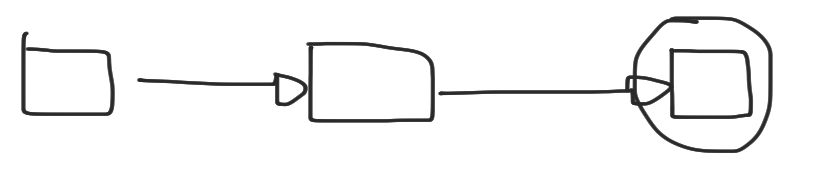
\includegraphics[scale=0.1]{content/graphics/game2}
(we can extend this for any natural number)\\
\textbf{3.} Enforce that the game ends after $\omega$ steps (you cannot bound it from below).
\footnote{
The smallest number of steps required for reachability game to finish is sometimes called the
\textbf{strength of a reachability game}.
}\\
We create such infinite graph:
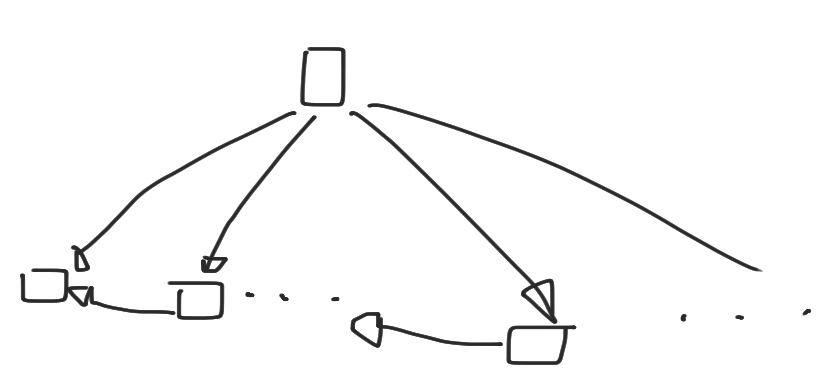
\includegraphics[scale=0.1]{content/graphics/game3}\\
\textbf{4.} Same for $\omega+1$ -- add one more $v_I$ to the previous graph\\
\textbf{5.} $\omega + \omega$ -- copy the graph, the output from first copy goes into the initial vertex of the second one\\

\noindent
$f : V \rightarrow V$\\
$f(S) = S'$, $S \subseteq S'$\\
$S' = \{v \in V\ |\ \forall_{v'} E(v,v') \rightarrow v' \in S\}
\cup \{v \in V\ |\ \exists_{v'} A(v,v') \rightarrow (v,v') \in E\} \cup S$\\
$f^{\alpha}(F) = S_{\alpha}$\\
$S_0 = F$\\
$S_{\alpha} \leftarrow$ set of winning positions of Eve\\
strenght of game = smallest $\alpha$ s.t. $v_I \in f^{\alpha}(F)$\\

\noindent
\textbf{6.} Given a reachability game $G = \langle V, W \rangle$, compute the set $W_E$ ($W_E = \{v\ |\ \text{Eve has a winning strategy from } v\}$).\\
\begin{lstlisting}
S = F;
S' = f(S);
while(S != S') {
 S = S';
 S' = f(S);
}
return S;
\end{lstlisting}

\subsection*{Parity games}
\textbf{Parity condition}:\\
$\{w \in \Gamma^{\omega}\ |\ w = a_0a_1a_2...a_n..., \lim\sup a_n \text{ is even }\}$ where $\Gamma \subseteq \mathbb{N}$\\
\textbf{Theorem}: Parity games are positionally determined.\\

\noindent
\textbf{7.} Let $G$ be a parity game, i.e. $G = \langle B, \textsc{Parity} \rangle$,
s.t. $V_A = \emptyset$ (only Eve moves). Compute the set of winning positions for Eve.\footnote{Since we are looking for an algorithm, assume graph $G$ is finite in size.}\\
\underline{Observation} $v \in V$ is a winning position iff we can reach from $v$ a loop $x_0...x_n$ s.t. the highest priority in the loop is even.
\underline{Proof}
\begin{itemize}
	\item[$\Leftarrow$] easy
	\item[$\Rightarrow$] $\exists \rightarrow$ $(v=v_1)v_2v_3...v_n...$ with ranks $a_1a_2a_3...a_n... \rightarrow$ winning. The highest priority occurring
	infinitely often is even, let's call it $a$.\\
	Thus $\underset{n_0}{\exists:} \underset{n \geq n_0}{\forall} a_n \leq a$\\
	Take a sequence $a_{n \geq n_0}...a...a....a....a$. So we choose a path between two occurrences of $a$ and loop it.
\end{itemize}
\textbf{HOME} Describe the algorithm basing on the observation.

\section{Lecture 4 (27 III 2019)}
\underline{Parity games}:
Eve wins a play $\pi = p_0p_1...$ if $\underset{n \rightarrow \infty}{\lim\sup} (rank(p_n))$ is even,
Adam otherwise.\\
\begin{figure}[H]
	\centering
	\caption{What are $W_E, W_A$ here? (squares are Adam, circles Eve)}
	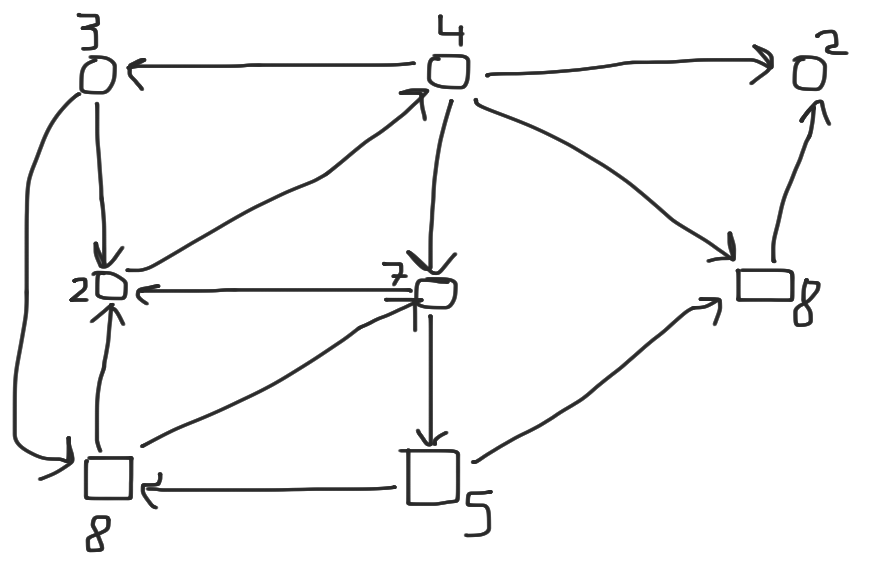
\includegraphics[scale=0.15]{content/graphics/game4}
\end{figure}
\noindent
\underline{General games on labelled graphs}:\\
$Pos_E, Pos_A, Move \in Pos \times Pos$\\
$rank\ :\ Pos \longrightarrow C$\\
Winning criteria:
$W_E \subseteq C^{\omega}, W_A \subseteq C^{\omega}, W_E \cap W_A = \emptyset$\\
\underline{Theorem}: Parity games are positionally determined. We prove for finite
arenas. Some positions are marked $\top$ immediately winning for Eve, $\bot$ immediately winning for Adam.
Induction on \#positions, not marked $\top, \bot$.\\
Induction step: Choose a position $p$ with the highest possible rank $d$, assume (wlog) $d$ is even.
\begin{itemize}
	\item[1] Suppose $p \in Pos_E$. Mark $p$ by $\top$.\\
	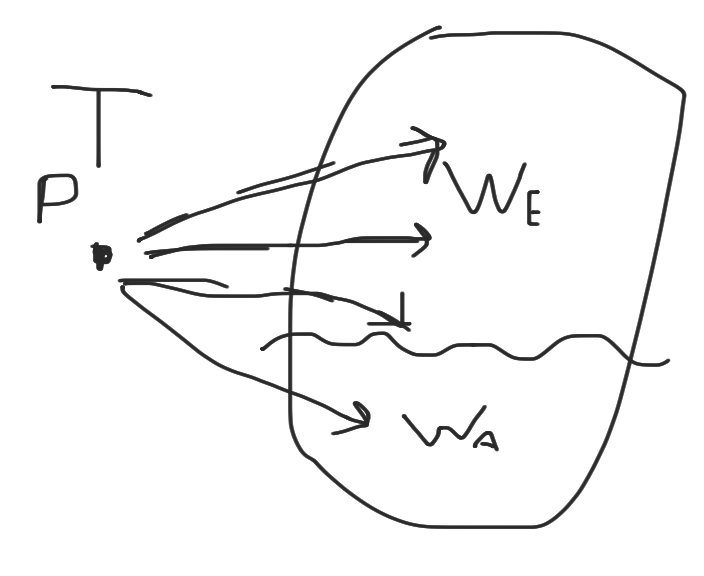
\includegraphics[scale=0.1]{content/graphics/game5}
	\begin{itemize}
		\item[(1a)] There is a move from $p$ to $W_E$.
		\item[(1b)] All moves from $p$ go to $W_A$.
	\end{itemize}
	\item[2] $p \in Pos_A$
	\begin{itemize}
		\item[(2a)] All moves from $p$ go to $W_E$.
		\item[(2b)] There is a move from $p$ to $W_A$.
	\end{itemize}
\end{itemize}

\noindent
Parity game -- $n$ vertices, $d$ ranks. "Simple" algorithm -- $n^{\frac{d}{2} + \Theta(1)}$

\section{Tutorials 5 (28 III 2019)}
\textbf{1.} \underline{Problem}\\
In: a parity game $G$ and a positional strategy of Eve $\sigma$\\
Out: is $\sigma$ winning?\\
$\sigma$ is winning $\leftrightarrow$ $\forall_{\pi} G(\sigma, \pi) \in \textsc{Parity}$\\
$\sigma\ :\ V \rightarrow V$\\

\noindent
\textbf{2.} In: a parity game $G$, and an initial position $v_I$.\\
Out: Is $v_I$ winning for Eve?\\
Solution in \textsc{NP}:
\begin{itemize}
	\item guess the positional strategy of Eve $\rightarrow \sigma_{p}$
	\item check if $\sigma_p$ is winning
\end{itemize}
Solution in \textsc{coNP} -- check for strategy for Adam.\\
The problem is (at least) in $\textsc{NP} \cap \textsc{coNP}$\\

\noindent
\textbf{3.}\\
Muller $C \subseteq \mathbb{N}, \mathcal{F} \subseteq 2^{C}$\\
$C^{\omega} \ni p = a_1a_2...a_n...$ if $Inf(p) \in \mathcal{F}$ $\longleftarrow$ set of letters in $p$ that appears $\infty$-often\\
Parity -- $max(Inf(p))$ is even
\begin{itemize}
	\item[1)] Parity is Muller
	\item[2)] Muller is \underline{not} positionally determined
	\item[3)] Muller is not Parity
	\item[4)] Show that Muller is determined, what is the required memory?
	Show that if $G$ is a Muller game, then for every initial vertex $v_I$, one of the players has a winning strategy.
\end{itemize}
Solutions:
\begin{itemize}
	\item[1)] Parity game of index $(i, k)$ can be represented as a Muller game, where $\mathcal{F}$ consists
	of subsets of $\{i, i+1, ..., k\}$ with even maximum.
	\item[2)] Example below:\\
	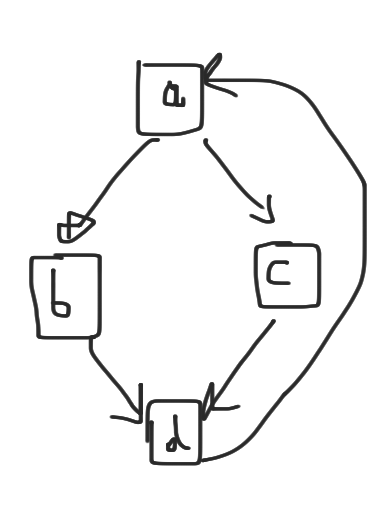
\includegraphics[scale=0.1]{content/graphics/game6}\\
	$\mathcal{F} = \{\{a, b, c, d\}\}$\\
	Every positional strategy removes either $b$ or $c$ and we require both.
	\item[3)] From (2)
	\item[4)] Idea: We will try to transform it to some Parity game, i.e.\\
	$G = \langle V, E, \lambda, v_I, \mathcal{F} \rangle \rightsquigarrow G^\prime = \langle V^\prime, E^\prime, \lambda^\prime, v_I^\prime, \textsc{Parity} \rangle$\\
	$E \subseteq V \times V$\\
	$\lambda\ :\ V \rightarrow C$\\
	s.t. $v_I$ is winning for Eve in $G \Leftrightarrow v_I'$ is winning for Eve in $G'$ (we need the same for Adam).
	In fact, we only need the implication to the left side.
\end{itemize}

\subsection*{LARs}
\textbf{LAR} (\textit{latest appearance record}) $w \in C \cup \{\natural\} (=\Gamma)$, every letter occurs at most once, $\natural$ occurs always.\\
$\textbf{up}\ :\ \text{LAR} \times \Gamma \rightarrow \Gamma$\\
$\textbf{up}(v_i \natural w_i, a) = \begin{cases}
	v_i \natural w_i a\ \ \ \ \ \ a \not\in v_i, a \not\in w_i\\
	[v_iw_i]_{a \mapsto \natural, \natural \mapsto \emptyset}a\ \ \ \ \text{else}
\end{cases}$

\noindent
\underline{Theorem}: The following cylindrification of $G$ is a solution to task (4):
$rank(p, v\natural a_1....a_l) = \begin{cases}
	2l\ \ \ \ \ \text{if} \{a_1,...,a_l\} \in \mathcal{F}\\
	2l + 1\ \ \ \ \ \text{otherwise}
\end{cases}$
\section{Lecture 6 (3 IV 2019)}
$G^{++}$\\
$\{0, 1, ..., n\}^{k+1} \approx k+1\text{-digit numbers in base }n+1$\\
Overflow = $(n+1)^{k+1}$\\

\noindent
$\textbf{up}(2i+1, \underbrace{a_0a_1a_2...a_k}_{m}) = m + (n+1)^{i}$\\
$\textbf{up}(2i, a_0a_1...a_k) = 0...0a_ia_{i+1}...a_k$\\

\noindent
$G^{++}$ is equivalent to $G$ (i.e. if Adam has winning strategy in $G$, he has
a winning strategy in $G++$)
\section{Tutorials 6 (4 IV 2019)}
\subsection*{Last week}
\underline{Theorem} If $G$ is a finite Muller game, then one of the players
has a finite memory winning strategy. $\langle V, E, v_I, \textsc{Muller} \rangle$\\
\underline{Proof} $G'$ -- a parity game s.t.\\
Adam wins in $G' \Rightarrow$ Adam wins in $G$\\
Eve wins in $G' \Rightarrow$ Eve wins in $G$\\
LARs
\subsection*{Automata}
$\mathcal{A} = \langle \Gamma, Q, q_i, \delta, F \rangle$\\
Word: $q_I \in Q, \delta: Q \times \Gamma \times Q, (q, a) \rightsquigarrow \{q_1, q_2, q_3, ...\}$\\
\subsubsection*{Infinite automata}
\textbf{Büchi condition} $F \subseteq Q$ (the states appearing infinitely often)\\
\textbf{Müller condition} $F \subseteq 2^Q$\\
\textbf{Parity}\\
\textbf{Safety} -- Parity with condition [0]\\
\underline{Theorem} Every regular language of infinite words is recognizable by a deterministic Müller
automaton.\\

\noindent
\textbf{1.}
Show that if $G$ is a finite Müller game, then set of plays is regular.\\

\noindent
$P$ -- set of plays\\
$P \subseteq V^\omega$\\
The automaton is the graph. $\langle V, V, v_I, \{ (v_1, v_2, v_3)\ |\ E \langle v_1, v_2 \rangle \} \rangle$\\

\noindent
\underline{Def} Game is $\omega$-regular if the winning condition is a regular set of winning plays.\\
$G = \langle V, L \rangle$. ($L \subseteq \Gamma^{\omega}$, Eve wins if $p \in L$)\\

\noindent
\textbf{2.}
Show that if $G$ is $\omega$-regular finite game then one of the players has a finite winning strategy.\\

\noindent
$G = \langle E, V_I, V_A, V_E \rangle, V = V_A \cup V_E$\\
$G_A = \langle V_A^\prime = V_A \times Q, V_E^\prime = V_E \times Q, V_I^\prime, E^\prime \rangle$\\
$G_A = \langle V^\prime, E^\prime, V_I^\prime \rangle$\\
$V^\prime = V \times Q$\\
$E^\prime = \{((v_1, q_1), (v_2, q_2))\ :\ (v_1, v_2) \in E, q_2 = \delta(q_1, v_1)\}$\\
$v_I^\prime = (v_I, q_I)$\\
$W = inf(L(P)) \in \mathcal{F}$\\
$L = \pi_2(p)$\\
\underline{Lemma}: $E$ has a finite memory winning strategy in $G_A$ $\Rightarrow$ $E$ has a
winning strategy in $G$.
\section{Lecture 7 (10 IV 2019)}
\begin{figure}[H]
    \centering
    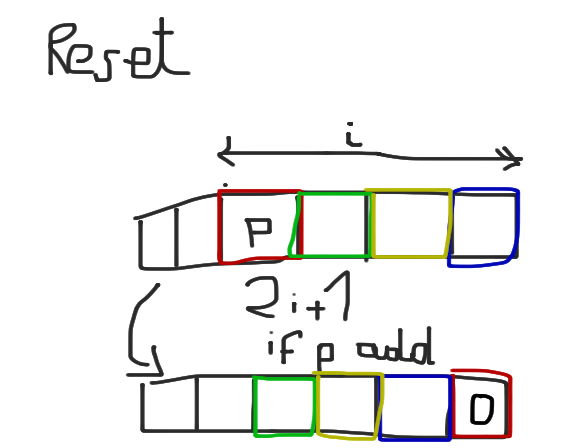
\includegraphics[scale=0.2]{content/graphics/game7.png}
\end{figure}
Parity games $n$, $\underbrace{d}_{rank}$.\\

\noindent
Karoliina Lehtinen -- algorithm.\\
$G$ -- a finite parity game.\\
We create a game $\mathcal{R}^E_k(G)$ with $k$ registers containing priorities $Mem \subseteq \{0, 1, ..., d\}^k$.
$\widetilde{Pos_E} = (Pos \times Mem \times \{0\}) \cup (Pos_E \times Mem \times \{1\})$\\
$\widetilde{Pos_A} = Pos_A \times Mem \times \{1\}$.\\

\noindent
If $p \rightarrow q$ in $G$ then\\
$(p, \alpha, 1) \xrightarrow[\text{1}] (q, up(\alpha), 0)$\\
$(p, \alpha, 0) \rightarrow (p, reset(\alpha), 1)$\\
$(p, \alpha, 0) \xrightarrow[\text{1}]{\text{[skip]}} (p, \alpha, 1)$\\

\noindent
$[up(\alpha)]_i = max(\alpha_i, rank(q))$\\

\noindent
\textbf{Lemma 1} If Adam wins original game $G$ from position $p$,
he wins $\mathcal{R}^E_k(G)$ from position $(p, \alpha, 1)$ for any number of registers $k$.\\
Adam plays the strategy from original game, we will show that any play is winning. Let $q$ be the maximal odd rank.
Let $i$ be the deepest register, which resets infinitely often. We will show, that infinitely often,
in the moment of reset of the register $i$, it contains $q$.\\

\noindent
\textbf{Lemma 2} If Eve wins the game $G$ from position $p$,
then $(\exists_k)$ Eve wins $\mathcal{R}^E_k(G)$ from position $(p, \alpha, 0)$.\\
$k$: number of ranks from the original game.\\
To each even rank $d$ we dedicate some register. When in original game there appears
an odd rank $d$, Eve resets the register dedicated to rank $d$.

\bibliographystyle{plain}
\bibliography{references}
\end{document}
